\documentclass[a4paper,11pt]{article}
\usepackage[margin=3.0cm]{geometry}
\linespread{1}
\usepackage[T1]{fontenc}
\usepackage[utf8]{inputenc}
\usepackage{lmodern}
\usepackage{tikz}
\usepackage{amsmath}
\usepackage{amsfonts}
\begin{document}

\begin{itemize}
\item[] \emph{u} : authenticated user
\item[] \emph{a} : authenticated admin
\item[] \emph{p} : posting
\item[] \emph{d} : deleting post(s)
\end{itemize}

\bigskip

Egenskap som gäller:
$$
{\cal M}_{\mathrm{Start}} \models \mathrm{AG}\:\mathrm{EF} (u \land p)
$$

Egenskap som inte gäller:
$$
{\cal M}_{\mathrm{Start}} \models \mathrm{AG} (\lnot d \lor \lnot u)
$$

% s0 = Start
% s1 = Logged in (user)
% s2 = Post_1
% s3 = Logged in (admin)
% s4 = Delete
% s5 = Post_2

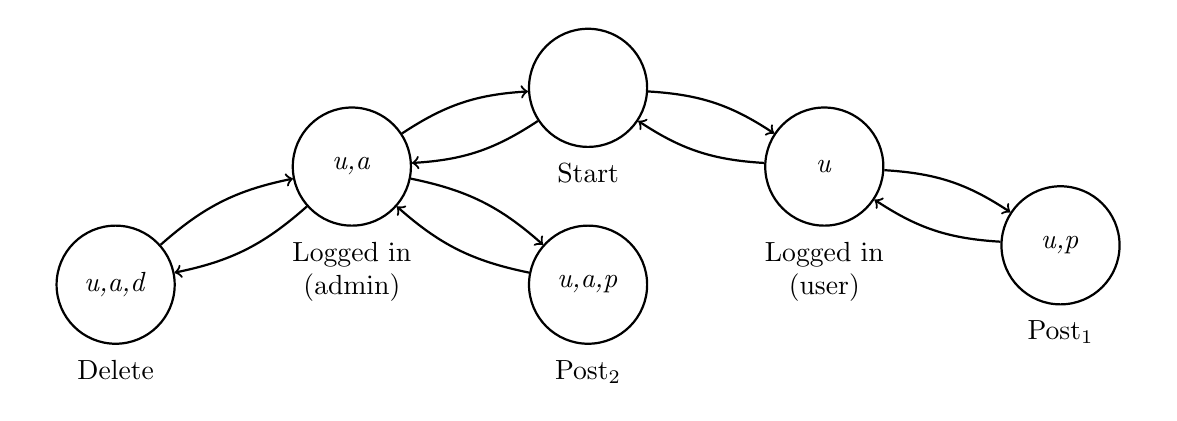
\begin{tikzpicture}
\node[label={[text width=2cm, align=center, below=1.6cm]Start},draw, thick, circle, minimum size=1.5cm] (start) at (0, 0) {};
\node[label={[text width=2cm, align=center, below=1.6cm]Logged in\\ (user)}, draw, thick, circle, minimum size=1.5cm] (authuser) at (3, -1) {\emph{u}};
\node[label={[text width=2cm, align=center, below=1.6cm]Post\textsubscript{1}}, draw, thick, circle, minimum size=1.5cm] (userpost) at (6, -2) {\emph{u,p}};

\node[label={[text width=2cm, align=center, below=1.6cm]Logged in\\ (admin)}, draw, thick, circle, minimum size=1.5cm] (authadmin) at (-3, -1) {\emph{u,a}};
\node[label={[text width=2cm, align=center, below=1.6cm]Post\textsubscript{2}}, draw, thick, circle, minimum size=1.5cm] (adminpost) at (0, -2.5) {\emph{u,a,p}};
\node[label={[text width=2cm, align=center, below=1.6cm]Delete}, draw, thick, circle, minimum size=1.5cm] (admindel) at (-6, -2.5) {\emph{u,a,d}};
% \draw (start) edge[out=12,in=110,->] (authuser);
% \draw[->] (start) to [out = 25, in = 90, looseness = 0.5] (authuser);
\draw[thick,->] (start) to [bend left=15] (authuser);
\draw[thick,->] (authuser) to [bend left=15] (start);
\draw[thick,->] (authuser) to [bend left=15] (userpost);
\draw[thick,->] (userpost) to [bend left=15] (authuser);

\draw[thick,->] (start) to [bend left=15] (authadmin);
\draw[thick,->] (authadmin) to [bend left=15] (start);
\draw[thick,->] (authadmin) to [bend left=15] (adminpost);
\draw[thick,->] (adminpost) to [bend left=15] (authadmin);
\draw[thick,->] (authadmin) to [bend left=15] (admindel);
\draw[thick,->] (admindel) to [bend left=15] (authadmin);
\end{tikzpicture}


\end{document}